\documentclass[11pt, aspectratio=169]{beamer}
\usetheme{Warsaw}
\usepackage[utf8]{inputenc}
\usepackage[english]{babel}


\author{A. Hoehne, A. M\"{o}slinger and E.F.M. Weterings}
\title{Are Comets the source of our water?}
\subtitle{Literature research into D/H ratio}
%\setbeamercovered{transparent} 
%\setbeamertemplate{navigation symbols}{} 
\logo{
\includegraphics[width=3cm]{figures/LTU_logo.jpg}} 
\newcommand{\nologo}{\setbeamertemplate{logo}{}} % command to set the logo to nothing
\institute{Lule\aa \ University of Technology} 
\date{17 October 2018} 
%\subject{} 
\begin{document}



\begin{frame}
\titlepage
\end{frame}

\begin{frame}[t]{Table of Contents}
\tableofcontents[
    currentsection,
    sectionstyle=show/show,
    subsectionstyle=show/show,
  ]
\end{frame}



\section{Formation comets \& asteroids}
\subsection{D/H ratio of asteroids and comets}
\begin{frame}[t]{D/H ratio of asteroids and comets}
Depends on:
\begin{itemize}
	\item position of creation
	\begin{itemize}
		\item Asteroid Belt
		\item Kuiper Belt
		\item Oort Cloud
	\end{itemize}
	\item for comets: behind the snow line
	\item time of creation
\end{itemize}
\end{frame}


\subsection{Timescale creation of comets}
\begin{frame}[t]{Timescale creation of comets}
\begin{figure}
	\centering
	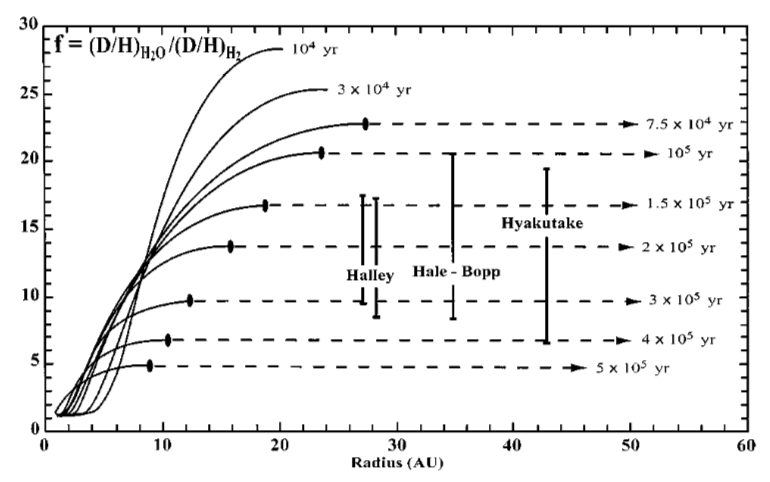
\includegraphics[height=0.7\textheight]{figures/D_H_distance_time}
\end{figure}
\end{frame}


\section{Creation terrestrial planets}
\subsection{Collisions protoplanets}
\begin{frame}[t]{Collisions protoplanets}
	\begin{columns}
	\begin{column}{0.5\textwidth}
		\centering
		\vspace{-1cm}
     	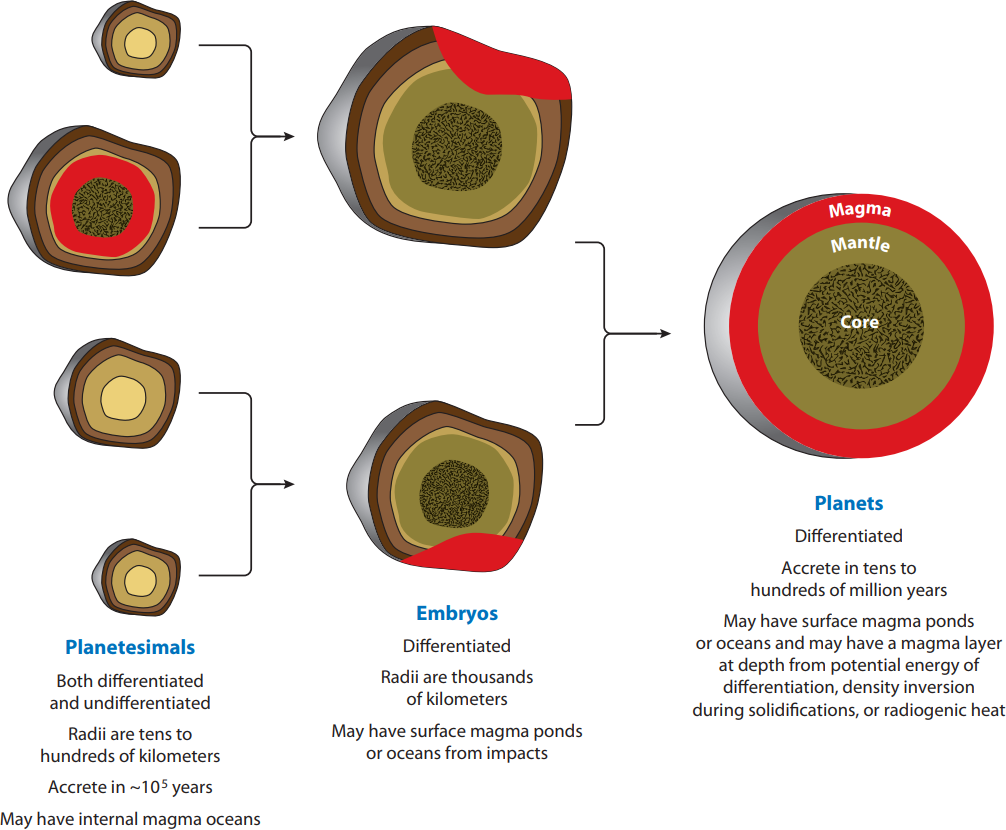
\includegraphics[height=.73\textheight]{figures/protoplanets.png} \\
     	\small (source: L. T. Elkins-Tanton, 2012)
	\end{column}
	\begin{column}{0.5\textwidth}
	\begin{enumerate}
		\item Volatile elements absorption onto grains due to:
		\begin{enumerate}
			\item Physisorption\\
			\item Chemisorption\\
		\end{enumerate}
		\item Volatile elements are stored inside the planetesimals.\\
		\item Volatile elements are released in the atmosphere due to magma ponds.\\
	\end{enumerate}
	\vspace{3cm}
	\end{column}
	\end{columns}	
\end{frame}


\subsection{Current D/H ratio of terrestrial planets}
\begin{frame}[t]{Current D/H ratio of terrestrial planets}
	\centering
	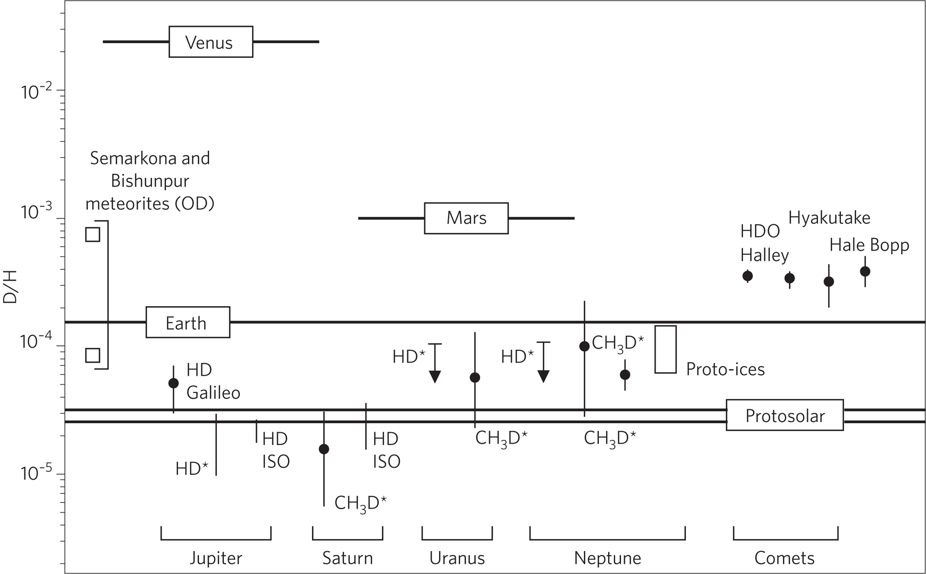
\includegraphics[height=.7\textheight]{figures/dh-ratio-terrestrial-planets.jpg}\\
	\small (source: A. Ingersoll, 2017)
\end{frame}



\section{Bombardment of Earth}
\subsection{Extra-Planetary Objects}
\begin{frame}[t]{Extra-Planetary Objects}
Comets
\begin{itemize}
	\item High Water Content
	\item Sufficient Quantities
	\item High D/H Ratio
\end{itemize}

Asteroids
\begin{itemize}
	\item Closer D/H Ratio
	\item Possibly Insufficient Quantities
	\item Questions Raised About Primordial Belt
\end{itemize}
\end{frame}


\subsection{Effects of Bombardment}
\begin{frame}[t]{Effects of Bombardment}
\begin{itemize}
	\item Atmosphere
	\item Plate Tectonics
	\item Lava Oceans
	\item Nuclear Winter
	\item Elevated Atmospheric Water Vapor
\end{itemize}
	
	
\end{frame}



\section{Questions}
\begin{frame}{Questions}
\centering
\Huge Thanks for listening\\

\huge Questions?\\\

\large A. Hoehne, A. M\"{o}slinger and E.F.M. Weterings\\

\end{frame}

\end{document}
